% !TeX root = ../../Parte1.tex
%\secmeme{html/headbody}
\subsection[Testo]{Semantica del testo}

\begin{frame}[fragile]{Enfasi del testo}\transfade\centering
  \htmlDual[-s A7][][trim={0 8.5cm 0 0},clip]{}{
        <em> Enfatizzato </em>
        <br>
        <strong> Importante </strong>
        <br>
        <mark> In evidenza </mark>
        <br>
        <del> Eliminato </del>
  }{}

\pause\bigskip
\alert{Attenzione!} non indicando lo stile del testo (italico, grassetto, evidenziato, sbarrato): quello lo faremo col CSS.

\pause\medskip
Esisterebbero dei tag HTML per definire lo stile, ma non andrebbrro mai usati.

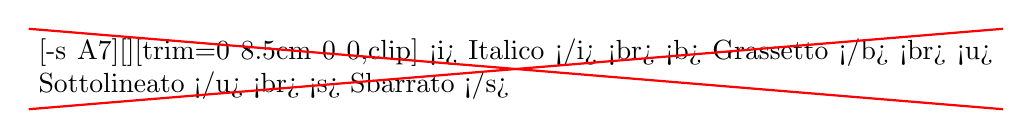
\begin{tikzpicture}
  \node (n1) {%
  \begin{minipage}{\textwidth}
    \htmlDual[-s A7][][trim={0 8.5cm 0 0},clip]{}{
        <i> Italico </i>
        <br>
        <b> Grassetto </b>
        <br>
        <u> Sottolineato </u>
        <br>
        <s> Sbarrato </s>
    }{}
  \end{minipage}%
  };
  \pause
  \draw[red, thick] (n1.south west) -- (n1.north east);
  \draw[red, thick] (n1.north west) -- (n1.south east);
\end{tikzpicture}

\end{frame}

\begin{frame}[fragile]{Apici e pedici}\transfade\centering
  \htmlDual[-s A7][][trim={0 8.5cm 0 0},clip]{}{
        1<sup>a</sup> classificata
        <br>
        H<sub>2</sub>O
  }{}
\end{frame}



\begin{frame}{Altri descrittori}\transfade\centering
  \begin{description}[<+->]
    \itemtt[small] Testo meno importante.
    \itemtt[cite] Citazione (riferimento).
    \itemtt[q] Citazione (testo citato).
    \itemtt[dfn] Definizione.
    \itemtt[abbr] Abbreviazione.
    \itemtt[time] Data e/o orario .
    \itemtt[codice] Codice sorgente.
    \itemtt[var] Variabile (matematica).
    \itemtt[samp] Output programma.
    \itemtt[kbd] Input programma, combinazione di tasti, percorso menù.
    \itemtt[wbr] Punto in cui si può andare a capo.
    \itemtt[span] blocco di testo generico (utile per applicare CSS).
  \end{description}
\end{frame}
